\subsection{Self-supervised Class-priors Estimation}
\label{sec:pi_estim}

As will be shown in our experiments, the optimization problem of Eq. \ref{eq:nnpu} requires frame-wise class-priors $\bm{\pi}$ to be effective.
As the latter parameter is unknown in the present scenario,
we devise a self-supervised strategy to estimate it from data.

In a nutshell, our approach works as follows.
We aim at finding for all frames an estimate of the true class-prior by iteratively training a prediction model with decreasing priors.
As initial priors, we consider an upper-bound.
After having trained our prediction model using the initial prior, we use the predictions of the same model as evidences to decrease the previous priors in a recursive bayesian fashion.
The latter two steps are repeated until a stopping condition is verified.

We first formalize our problem as a state-space model.
Next, we describe how the latter can be solved using the recursive bayesian estimation paradigm.
Last, we suggest a stopping condition.

\subsubsection{State-space model}

Let $\bm{\tilde\pi}_k=\{\tilde\pi_{k}^{i}\}_{i=1}^N$,
the hidden state variable representing the class prior at time $k$.
Furthermore, let $\hat \pi_0 > \pi^{i}, \forall i$ an initial upper-bound on the true prior.
We consider a model that provides \(\bm{\rho}_k=\{\rho_{k}^i\}_{i=1}^N\), a noisy observation of $\bm{\tilde\pi}_{k}$.
Our idea is to progressively decrease $\bm{\tilde\pi}_{k}$ from its initial value $\hat \pi_{0}$ by using $\bm{\rho}_{k}$ as observations.
We introduce the following state-space model:

\begin{align}
\bm{\bm{\tilde\pi}}_{k+1} &= g(\bm{\tilde\pi}_{k}, L) - u_{k}\mathbf{1}_{N} + \mathcal{N}(0,Q), \quad \tilde\pi_{k}^{i} \in [0; \pi_{{max}}] \label{eq:trans_fn}\\
\bm{\bm{\rho}}_{k} &= \bm{\tilde\pi}_{k} + \mathcal{N}(0,R) \label{eq:proc_fn} \\
\bm{\tilde\pi}_{0}&=\hat \pi_{0} + \mathcal{N}(0,S) \label{eq:init_fn}
\end{align}

Where $Q$, $R$, and $S$ are the transition, observation, and initial covariance matrices, respectively.
The function $g(., L)$ is a moving average filter of length $L$ with a Hanning window which imposes a frame-wise smoothness.
For convenience, we write $\mathbf{1}_{N}$ for a vector of length $N$ taking values of $1$.
The term $u_{k}$ is the control input:
\begin{equation}
u_{k} = u_{0} + (u_{T} - u_{0})\frac{k}{T}
\end{equation}

Where $u_{0}$ and $u_{T}$ two constants such that $u_{T} > u_{0}$.
This term therefore induces a downward acceleration on the states and imposes a ``sweeping'' effect on the latter, which allows in principle the range $[0; \hat \pi_{0}]$ to be explored.

\subsubsection{Observation model}
\label{sec:obs_model}
We are now interested in inferring robust obervations from our prediction model.
For clarity, we write $f_{\theta_{k}}$ for our prediction model trained for $k$ epochs.
Let $f_{\theta_{k}}(x)$ the prediction given by $f_{\theta_{k}}$ on superpixel $x$ at iteration $k$.
We therefore compute $\rho_{k}^{i}$, the observation at time $k$ on frame $i$ as:

\begin{equation}
  \label{eq:observ}
\rho_{k}^{i} = \mathbb{E}_{x \in \mathcal{X}^{i}}[f_{\theta_{k}}(x)^{\gamma}]
\end{equation}

With $\gamma > 1$ a correction factor.
This correction is justified as follows: As early iterations use class-priors that are above the true values,
our prediction model tends to over-segment the object of interest and therefore over-estimate the frequencies of positives.

\subsubsection{Recursive Bayesian Estimation}
Our ultimate goal is to obtain an optimal estimate of our state.
As criterion of optimality, we choose the mean-squared error.
The optimal state estimate is therefore given by the conditional mean:

\begin{equation}
  \label{eq:cond_mean}
\bm{\hat\pi}_{k} = \mathbb{E}[\bm{\tilde \pi}_{k} | \bm{\rho}_{0:k}]
\end{equation}

Where $\bm{\hat\pi}_k$ is the optimal estimate of $\bm{\tilde\pi}_{k}$ given $\bm{\rho}_{0:k}$, the sequence of observations from time $0$ to $k$.
The latter conditional expectation requires the knowledge of the a posteriori probability density function (PDF) $p(\bm{\tilde\pi}_{k}|\bm{\rho}_{0:k})$.
Using Bayes' rule, we write:
\begin{equation}
  \label{eq:aposteriori}
  p(\bm{\tilde\pi}_{k}|\bm{\rho}_{0:k}) = \frac{p(\bm{\tilde\pi}_{k}|\bm{\rho}_{0:k-1})\cdot p(\bm{\rho}_{k}|\bm{\tilde\pi}_{k})}{p(\bm{\rho}_{k}|\bm{\rho}_{0:k-1})}
\end{equation}

Where
\begin{equation}
  \label{eq:prior}
  p(\bm{\tilde\pi}_{k}|\bm{\rho}_{0:k-1}) = \int p(\bm{\tilde\pi}_{k}|\bm{\tilde\pi}_{k-1}) \cdot p(\bm{\tilde\pi}_{k-1}|\bm{\rho}_{0:k-1}) d\bm{\tilde\pi}_{k-1}
\end{equation}

is a recursive expression of the state PDF at time $k$ as a function of the state PDF at time $k-1$, and the most recent observations.
The bottom term of Eq. \ref{eq:aposteriori} is a normalization factor that writes:

\begin{equation}
  \label{eq:norm_cst}
  p(\bm{\rho}_{k}|\bm{\rho}_{0:k-1}) = \int p(\bm{\tilde\pi}_{k}|\bm{\rho}_{0:k-1}) \cdot p(\bm{\rho}_{k}|\bm{\tilde\pi}_{k}) d\bm{\tilde\pi}_{k}
\end{equation}

Our state-space model provides expressions of the state-transition probability $p(\bm{\tilde\pi}_{k}|\bm{\tilde\pi}_{k-1})$ via Eq. \ref{eq:trans_fn}, and likelihood $p(\bm{\rho}_{k}|\bm{\tilde\pi}_{k})$ via Eq. \ref{eq:proc_fn}.

In a recursive bayesian filtering application, one distinguishes two phases: prediction and update, where the prediction phase computes the a-priori state density (Eq. \ref{eq:prior}) using the transition function.
In the update phase, a new observation vector is available that allows to compute the likelihood $p(\bm{\rho}_{k}|\bm{\tilde\pi}_{k})$ and normalization constant of Eq. \ref{eq:norm_cst}.
Last, the a-posteriori state estimate is computed using Eq. \ref{eq:aposteriori}.

Modeling the states as a multi-variate gaussian random variable (GRV) with additive gaussian noise greatly simplifies the computation of Eq. \ref{eq:prior} and \ref{eq:norm_cst}.
Assuming further that the transition and observation models are linear, one typically resort to the trusted Kalman Filter (KF) \cite{kalman1960}.

However, the present scenario imposes an inequality constraint on the states so as to make them interpretable as probabilities, a requirement that standard KF does not handle.
In \cite{gupta07}, authors suggest to apply an intermediate step in which the a-priori state estimates are projected on the constraint surface.
This approach, despite being effective, requires the solving of a quadratic program at each iteration.

Our solution follows the simpler approach of \cite{kandepu08}, who relie on the Unscented Kalman Filter (UKF) approach \cite{wan00}.
In contrast with standard KF, which propagate the means and covariances of states through the (linear) system, UKF samples a set of carefully chosen points from the state distribution, called sigma-points, that allow to accurately approximate the true statistics of the posterior.
Our inequality constraints are then directly applied to the sigma-points.
% TODO: introduce capital pi

\subsubsection{Stopping condition}
By construction, our state-space model tends to force the states to decrease, and often to go past below the true values.
We therefore devise a composite stopping condition.

Let $\bm{\tilde{\mathcal{X}}}_{n}=\{x \in \bm{\mathcal{X}} | f_{\theta}(x) < 0.5\}$, and $\bm{\tilde{\mathcal{X}}}_{p}=\{x \in \bm{\mathcal{X}} | f_{\theta}(x) \geq 0.5\}$ the set of ``pseudo-negative'' and ``pseudo-positive'' superpixels, respectively.
As a first criteria, we use the variance of the predictions of  $\bm{\tilde{\mathcal{X}}}_{n}$, written $Var[f_{\theta}(\bm{\mathcal{\tilde X}}_{n})]$, which gives a measure of the confidence of our model on the background.
Second, we also impose that our predictions are such that the frequency of positives is below our upper-bound on all frames.
Concretely, our composite stopping criteria are:

\begin{enumerate}
\item Impose a maximum on the frequencies of pseudo-positives, i.e. $\frac{|\bm{\tilde \mathcal{X}}_{p}^{i}|}{N_{i}} < \hat \pi_{0} \quad \forall i$.
\item Impose a maximum variance level to pseudo-negatives, i.e. $Var[f_{\theta}(\bm{\mathcal{\tilde X}}_{n})] < \tau$.
\end{enumerate}

In practice, we want the above conditions to be verified for several iterations so as to guarantee stability.
We therefore impose that these conditions are verified for $T_{s}$ iterations.
In particular, we denote $C(\bm{\hat \pi}_{k})$ a boolean function that represents the above conditions, and select the optimal prior $\bm{\hat \pi}^{*}$ as

\begin{equation}
  \label{eq:prior_opt}
  \bm{\hat \pi}^{*} = \bm{\hat \pi}_{k} \quad \text{iff} \quad C(\bm{\hat \pi}_{k}) \wedge
  C(\bm{\hat \pi}_{k+1})
  \wedge \cdots \wedge  C(\bm{\hat \pi}_{k+T_{s}})
\end{equation}


\begin{algorithm}[H]
\caption{Self-supervised class-prior estimation}
\label{alg:prior_estim}
\begin{algorithmic}
\Require{$\hat \pi_{0}$: Upper-bound on class-priors} \newline
  $T$: Number of epochs \newline
  $f_\theta$: Foreground prediction model
\Ensure {Optimal estimate of class-prior $\bm{\hat{\pi}}^{*}$}
\State $k \gets 0$
\While {Stopping condition is not verified}
    \State Optimize $f_\theta$ for $1$ epoch as in Alg. \ref{alg:sgdnnpu} using priors $\bm{\hat{\pi}}_{k}$
    \State Forward pass all images to get $\bm{y}_k$
    \State Compute observations $\bm{\rho}_k$ from $\bm{y}_{k}$ as in Eq. \ref{eq:observ}
    \State Clip $\bm{\rho}_{k}$ to $[0,\hat \pi_{0}]$
    \State Denote $\bm{\hat\Pi}_{k-1}$ the sigma-points of $\bm{\hat\pi}_{k-1}$
    \State Clip $\bm{\hat\Pi}_{k}$ to $[0, \hat \pi_{0}]$
    \State Transform $\bm{\hat\Pi}$ through the state-transition function to get $\bm{\hat\Pi}_{k+1}^{-}$
    \State Clip $\bm{\hat\Pi}_{k+1}^{-}$ to $[0, \hat \pi_{0}]$
    \State Compute a-posteriori state $\bm{\hat\pi}_{k+1}$ using observations $\bm{\rho}_{k}$
    \State $k \gets k+1$
\EndWhile
\end{algorithmic}
\end{algorithm}

Alg. \ref{alg:prior_estim} summarizes our approach.
On Fig. \ref{fig:prevs_conv}, we illustrate its behaviour by showing the predicted probabilities and their corresponding class-priors for a Brain sequence.

\begin{figure*}[t]
\caption{Visual example of our self-supervised class-prior estimation. (Top row): Original image with groundtruth highlighted in red and 2D location in green, output prediction at different epochs. (Bottom row): Priors at corresponding epochs. The true priors are in blue, observations are in orange, frequencies of classifier are in green, and current state estimate is in red.}
\centering
    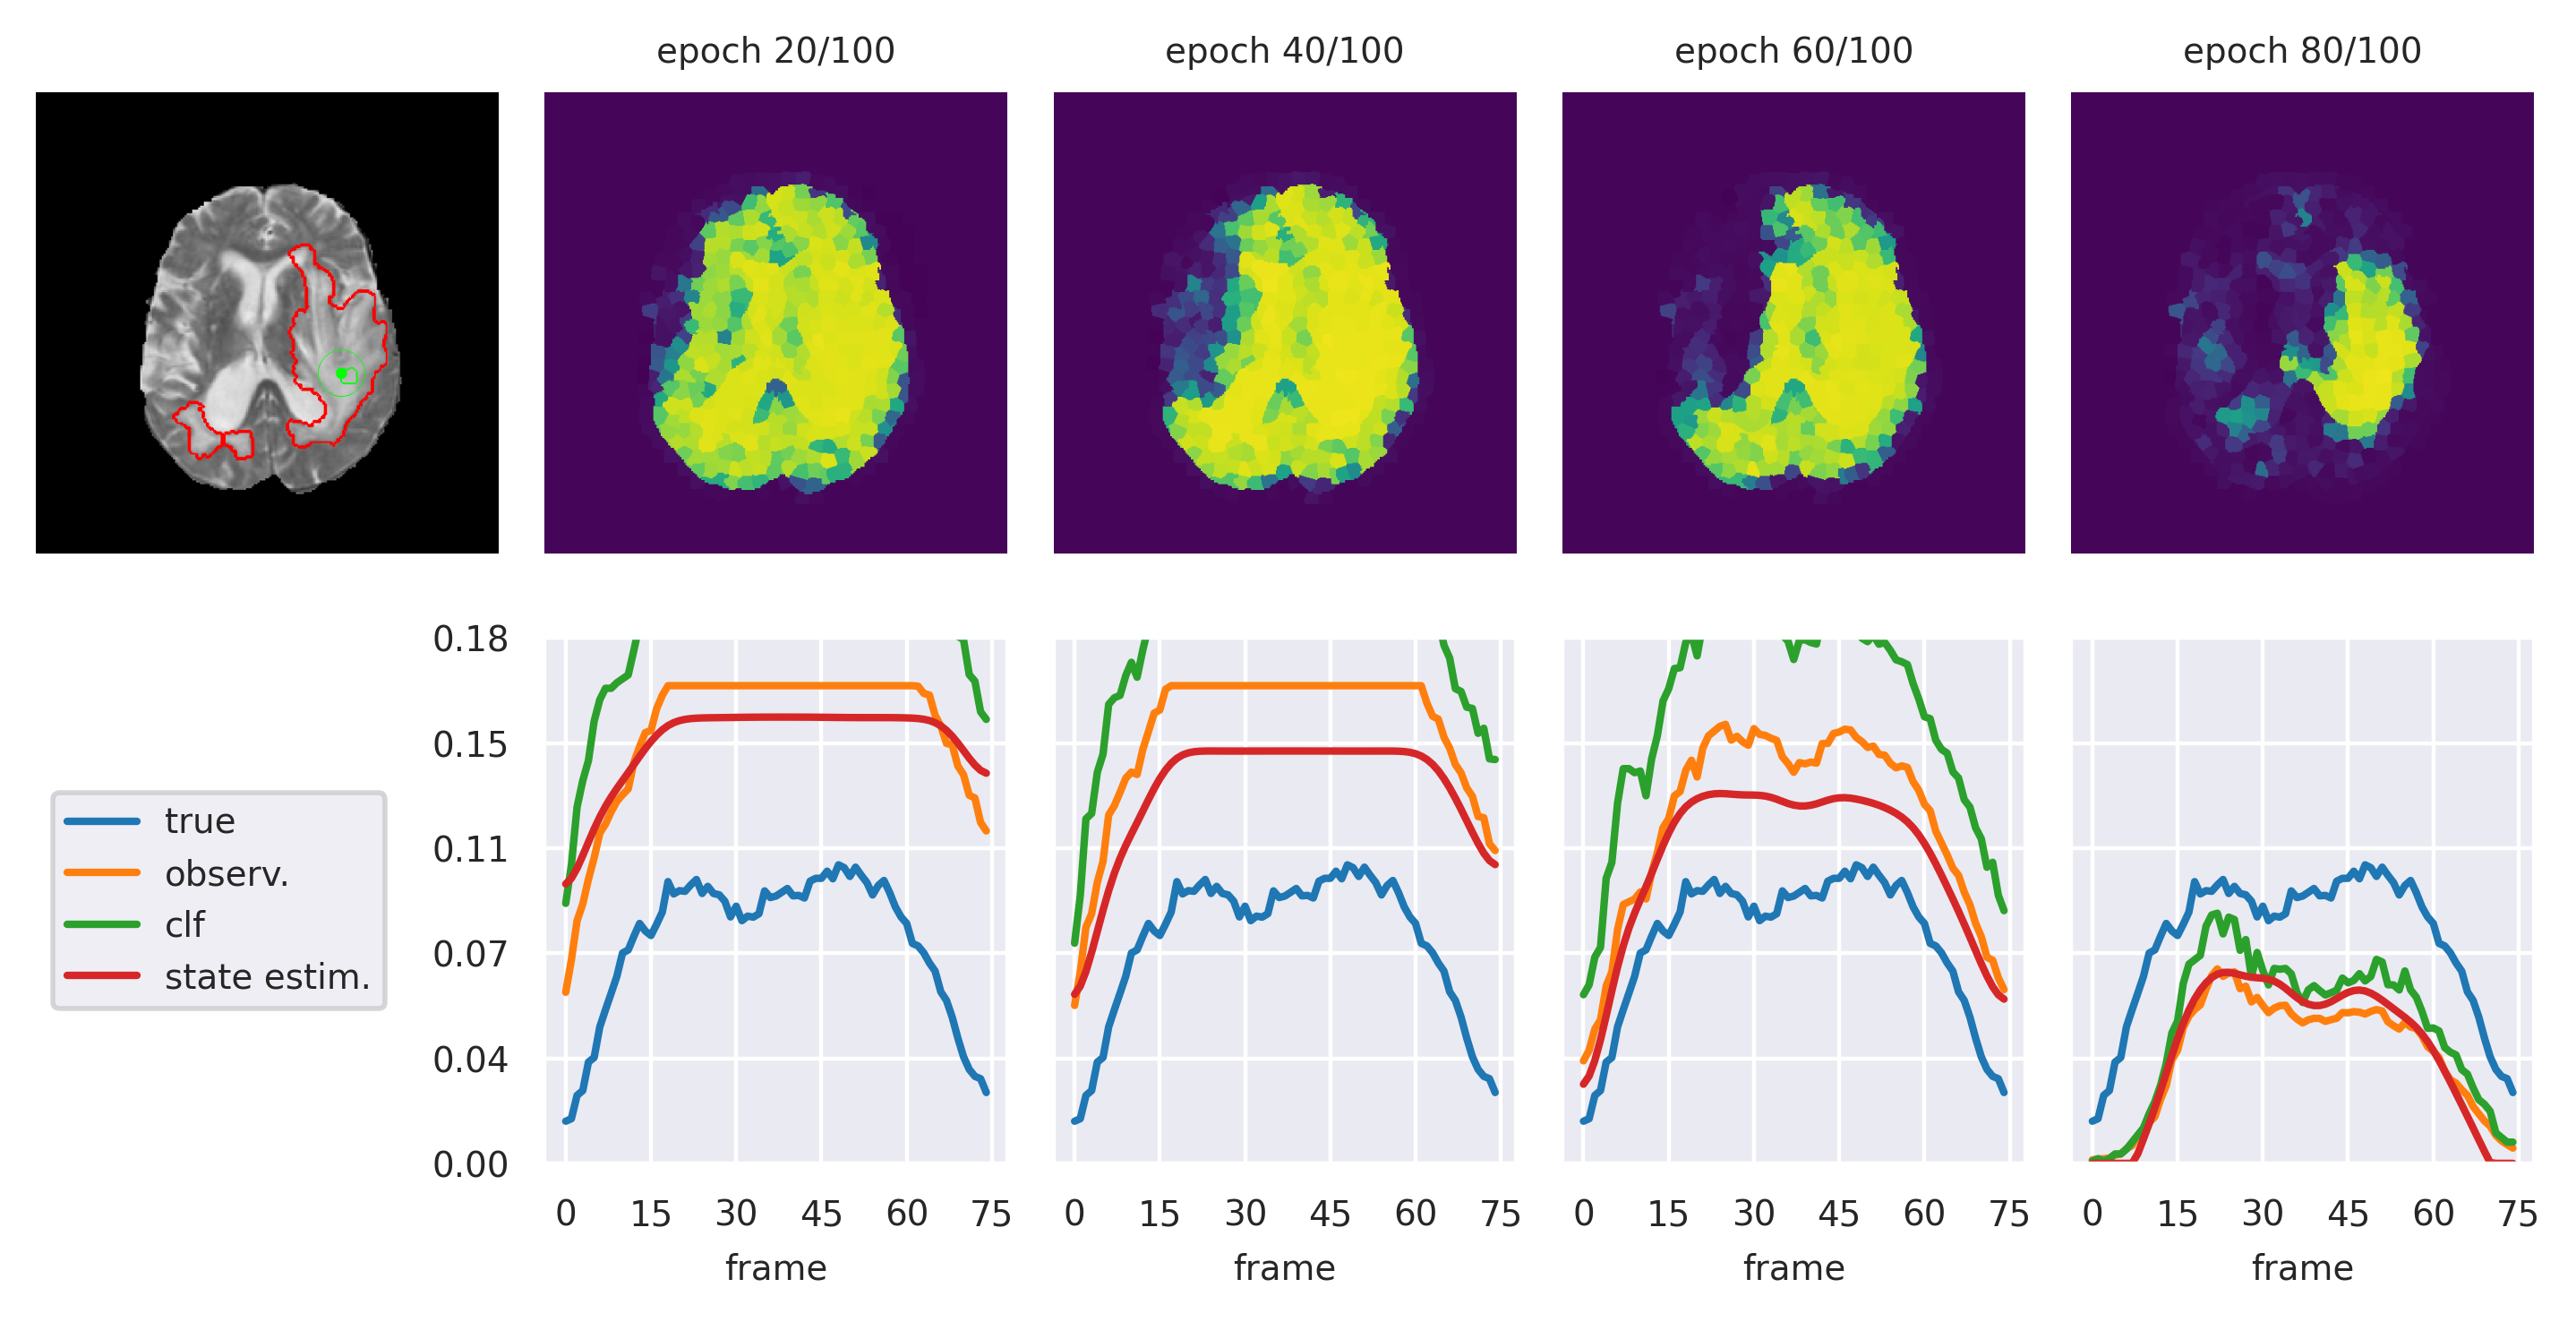
\includegraphics[width=.9\textwidth]{pics/prevs_conv.png}
\label{fig:prevs_conv}
\end{figure*}


%%% Local Variables:
%%% mode: latex
%%% TeX-master: "main"
%%% End:
